%!TEX root = ../Principal.tex
%Capa do Trabalho
\imprimircapa

%Folha de Rosto
%* indica que tem ficha catalográfica
\imprimirfolhaderosto*

% ---
% Caso a Biblioteca da UDESC forneça, utilize o comando
% ---
% \begin{fichacatalografica}
%     \includepdf{fig_ficha_catalografica.pdf}
% \end{fichacatalografica}

% ---
% Geração da Ficha Catalográfica Via LaTeX
% ---
\begin{fichacatalografica}
	\vspace*{\fill}					% Posição vertical
	\begin{center}					% Minipage Centralizado
	\begin{minipage}[c]{12.5cm}		% Largura
	
	\imprimirautor
	
	\hspace{0.5cm} \imprimirtitulo  / \imprimirautor. --
	\imprimirlocal, \imprimirdata-
	
	\hspace{0.5cm} \pageref{LastPage} p. : il. (algumas color.) ; 30 cm.\\
	
	\hspace{0.5cm} \imprimirorientadorRotulo~\imprimirorientador\\
	
	\hspace{0.5cm}
	\parbox[t]{\textwidth}{\imprimirtipotrabalho~--~\imprimirinstituicao,
	\imprimirdata.}\\
	
	\hspace{0.5cm}
		1. Tópico 01.
		2. Tópico 02.
		I. Prof. Dr. xxxxx.
		II. Universidade do Estado de Santa Catarina.
		III. Centro de Ciências Tecnológicas.
		IV. identificação xxxx\\ 			
	
	\hspace{8.75cm} CDU 02:121:005.7\\
	
	\end{minipage}
	\end{center}
\end{fichacatalografica}

% ---
% Folha de Aprovação
% ---
% Exemplo de folha de aprovação antes da Banca. Após isso, incluia o pdf digitalizado com as assinaturas%
% 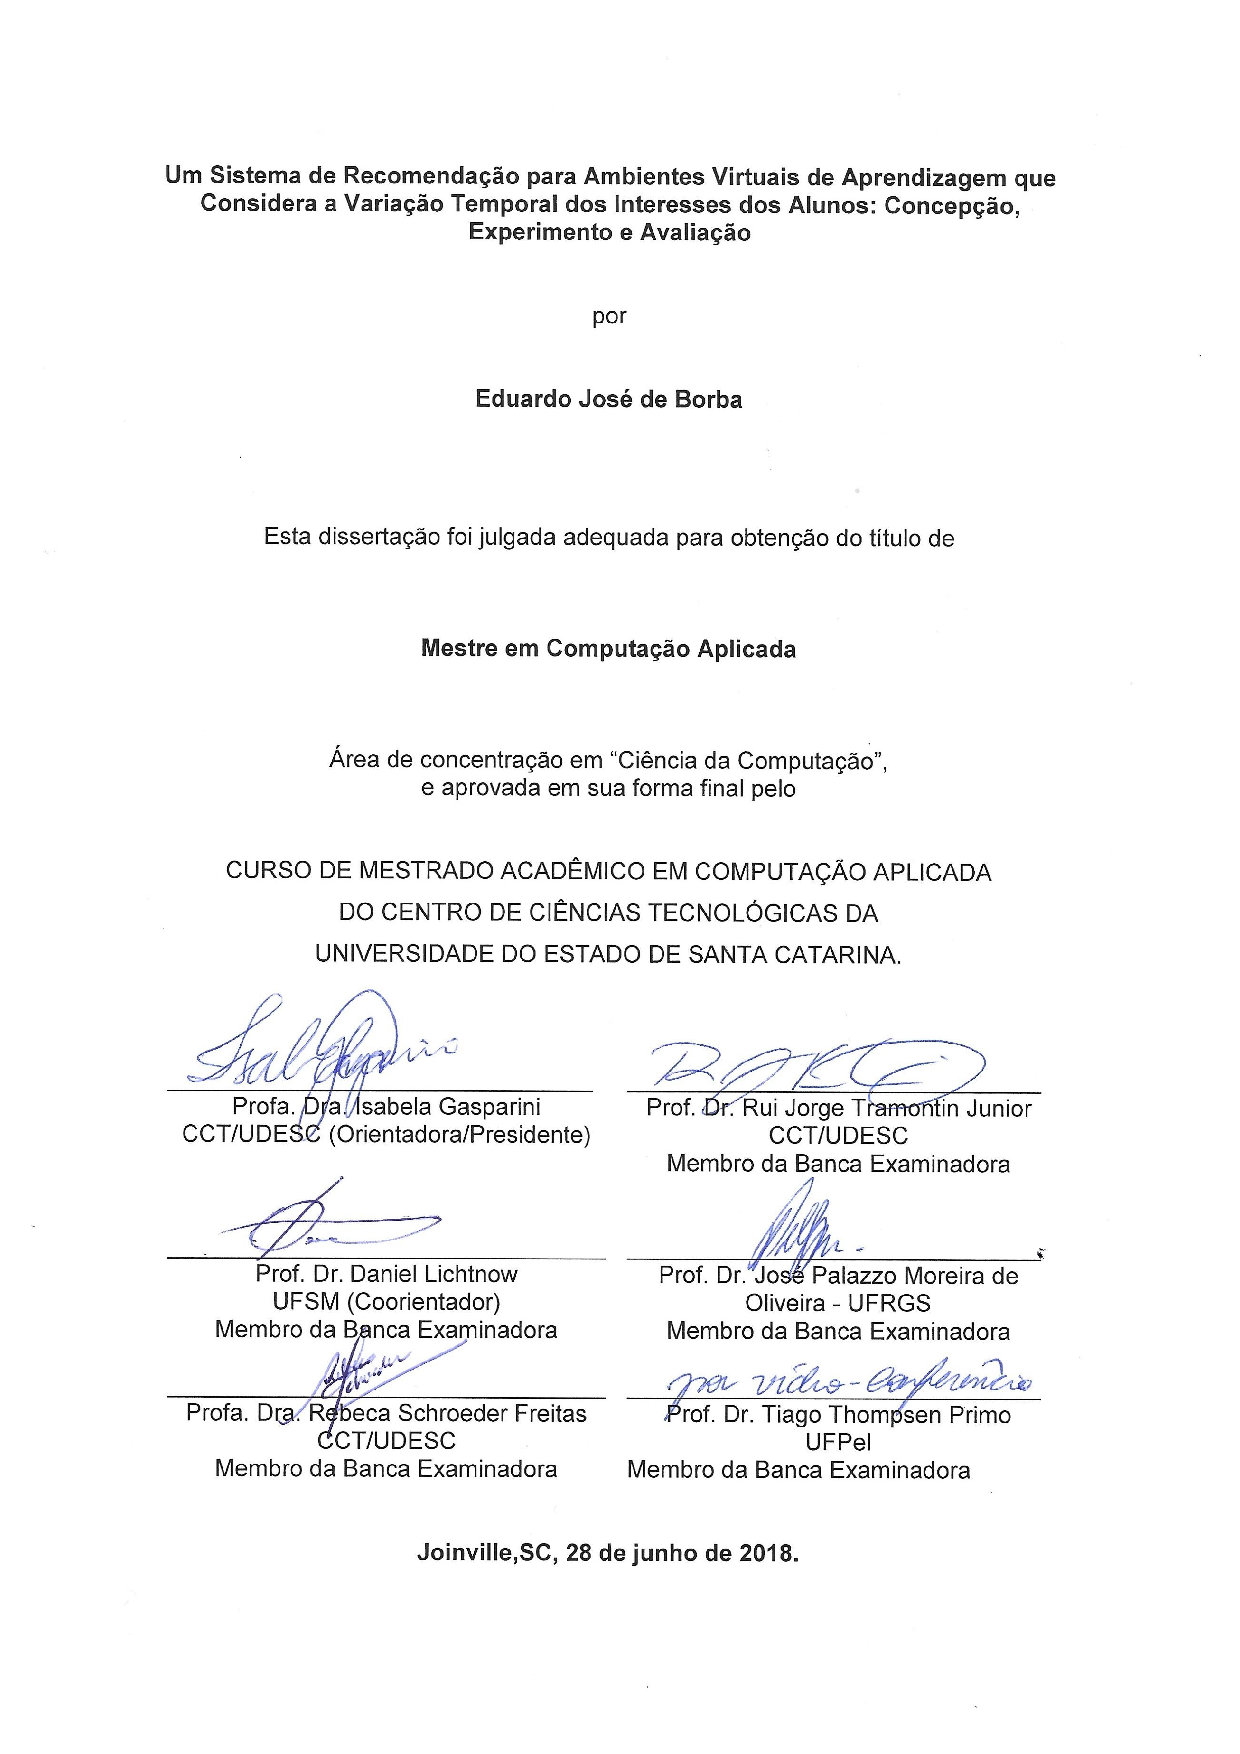
\includepdf{folhadeaprovacao_final.pdf}
\begin{folhadeaprovacao}

	\begin{center}
		{\ABNTEXchapterfont\bfseries\imprimirautor}
		\vspace{6em}

			\ABNTEXchapterfont\bfseries\imprimirtitulo
		
	\end{center}
		\vspace{1em}
		{\justify
		Esta dissertação foi julgada adequada para a obtenção do título de
    	{\ABNTEXchapterfont\bfseries Mestre em Computação Aplicada}   
   		área de de concentração em "Sistemas de Computação",
   		 e aprovada em sua forma final pelo Curso de Mestrado em Computação Aplicada do Centro
   		 de Ciências Tecnológicas da Universidade ddo Estado de Santa Catarina.}
	
	\vspace{3em} 
	\noindent
	{\bfseries Banca Examinadora:}
	\assinatura{\textbf{\imprimirorientador} \\ Orientador} 
	\assinatura{\textbf{Professor} \\ Convidado 1}
    \assinatura{\textbf{Professor} \\ Convidado 2}
    \assinatura{\textbf{Professor} \\ Convidado 3}

    \vspace*{\fill}
    \begin{center}
    	\imprimirlocal,\,\imprimirfulldata
    \end{center}
\end{folhadeaprovacao}

% ---
% Dedicatória
% ---
\begin{dedicatoria}				
Dedico este trabalho aos meus familiares, amigos, colegas e professores que me acompanharam e me deram forças nessa magnífica trajetória.  
\end{dedicatoria}

% ---
% Agradecimentos
% ---
\begin{agradecimentos}
Gostaria de agradecer...

Aqui devem ser colocadas os agradecimentos às pessoas que de alguma forma contribuíram para a realização do trabalho.
\end{agradecimentos}

% ---
% Epígrafe
% ---
\begin{epigrafe}	
``Independentemente das circunstâncias, devemos ser sempre humildes, recatados e despidos de orgulho.''
\\
\par
Dalai Lama 
\end{epigrafe}

% ---
% RESUMOS
% ---

% Português
\begin{resumo}
 O resumo deve ressaltar o
 objetivo, o método, os resultados e as conclusões do documento. A ordem e a extensão
 destes itens dependem do tipo de resumo (informativo ou indicativo) e do
 tratamento que cada item recebe no documento original. O resumo deve ser
 precedido da referência do documento, com exceção do resumo inserido no
 próprio documento. (\ldots) As palavras-chave devem figurar logo abaixo do
 resumo, antecedidas da expressão Palavras-chave:, separadas entre si por
 ponto e finalizadas também por ponto.

 \vspace{\onelineskip}
    
 \noindent
 \textbf{Palavras-chaves}: latex, abntex e editoração de texto.
\end{resumo}

% Inglês
\begin{resumo}[Abstract]
 \begin{otherlanguage*}{english}
	Resumo em inglês
   \vspace{\onelineskip}
 
   \noindent 
   \textbf{Key-words}: latex, abntex e text editoration.
 \end{otherlanguage*}
\end{resumo}

% ---
% Lista de Figuras
% ---
\pdfbookmark[0]{\listfigurename}{lof}
\listoffigures*
\cleardoublepage
% ---

% ---
% Lista de Tabelas
% ---
\pdfbookmark[0]{\listtablename}{lot}
\listoftables*
\cleardoublepage